The metal films were deposited directly on substrates by means of a plasma
sputtering process.  It is through this process that the surface roughness
of the metal film was also controlled.  Our base process consists of
top-down sputtering in Argon plasma at a pressure of \SI{1}{\milli\torr}
and a flow rate of \SI{12}{STP}.  The deposition rates were
\SI{6.60}{\angstrom\per\second} for gold and
\SI{5.88}{\angstrom\per\second} for silver at 150 and \SI{66}{\watt} DC,
respectively.  During sputtering, the samples were rotated at \SI{50}{RPM}.
Adhesion of the metal films to both glass and fluoropolymer substrates was
found to be very poor, but we did not attempt to address this issue.
Instances of film-substrate separation were rare enough (4-5 times amongst
hundreds of experiments) that it did not warrant the effort given our
careful attention to stresses on the film.  Typical surface qualities are
shown in \Figure{fig:semsputter} for both gold and silver.  
\begin{figure}
\centering
\includegraphics[keepaspectratio,width=5cm]{experimental/figures/SEM-nanoparticles.pdf}
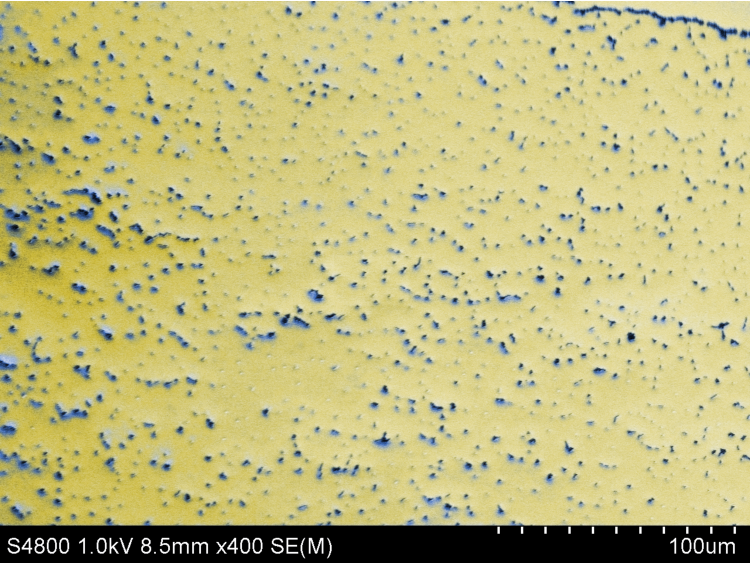
\includegraphics[keepaspectratio,width=5cm]{experimental/figures/SEM-holesa.pdf}
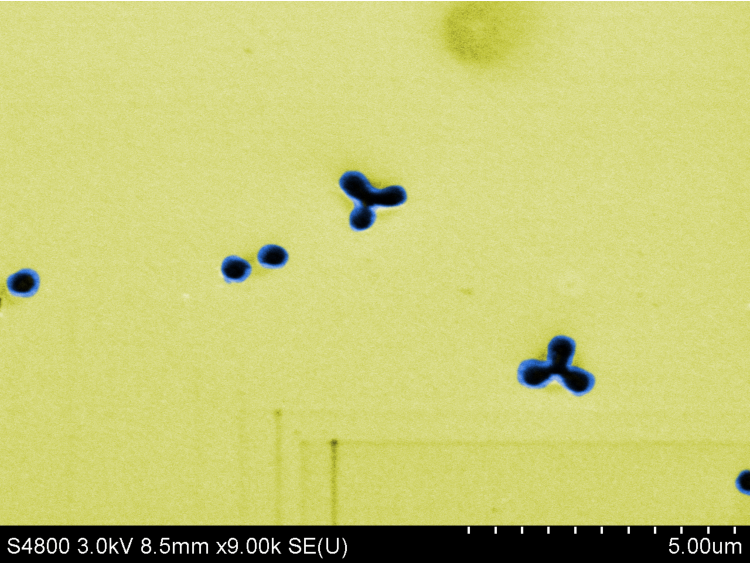
\includegraphics[keepaspectratio,width=5cm]{experimental/figures/SEM-holesb.pdf}
\caption{SEM images of typical films produced with the plasma sputtering
technique using the base set of parameters described in the text.}
\label{fig:semsputter}
\end{figure}

The substrate material consisted of \SI{12}{\milli\meter} diameter BK7
glass slides with nominal surface roughness of XXX.  They were cleaned in
the following way.  A \SI{2}{\percent} solution of Hellmanex II was first
prepared in a pyrex beaker with a volume of \SI{25}{\milli\liter} and
heated to a temperature of \SI{60}{\celsius} on a hot plate.  The BK7
slides are placed in this solution on the hot plate and washed for
\SI{300}{\second}, swirling gently by hand occasionally.  The container
with the solution and slides was then sonicated for \SI{300}{\second}.
After sonication, the slides are removed from the solution and washed
liberally with distilled water and dried under a nitrogen stream.  Cleaned
glass slides were stored individually on top of a small
\SI{1}{\milli\meter\cubed} piece of PDMS plasma bonded to a microscope
slide, and batches kept in a dark box until use.  Slides sputtered with
metal films were stored in the same manner, but always used within one week
of preparation.

Once deposited, whilst a gold film will last virtually forever if left
undisturbed, the silver film should slowly lose its integrity due to
oxidation.  This has not been observed, as new films are easily created at
regular intervals.  

Since the metal films are very thin and SPR is particularly sensitive to
surface conditions, care must be taken not to damage the films.  Once
prepared, they cannot be touched in any way.  Cleaning them with lens
tissue, even using the drag and drop method, destroys their integrity.  Dry
nitrogen seems to be the only option for removing dust if contaminated, but
prevention is always preferable.

\subsection{Prisms}
Several different types of hemispherical prisms were used during the
experimental work.  The first iteration used \SI{10}{\milli\meter} LAH79 or
BK7 glass hemispheres upon which the metal was deposited directly.  The
prisms were prepared as follows.  First, any existing metal film was
removed.  Silver films were removed by immersion in \SI{70}{\percent}
\ce{HNO3} for \SI{60}{\second}.  Gold films were removed by immersion in
freshly prepared aqua regia, composed of a 1:3 ratio of \ce{HNO3} to
\ce{HCl}.  Second, the prisms were sonicated in acetone to remove any
organic contaminants and rinsed in ultra-pure dry acetone.  The surface was
then cleaned with methanol and lens tissue using the drag and drop method.

For reasons of experimental convenience, we also fabricated disposable
hemispheres using NOA89 optical UV adhesive.  To do this, BK7 glass
hemispheres were immersed in PDMS to create a mould.  Once the glass
hemisphere was removed, the void was filled with NOA89 and cured under a
\SI{15}{\watt} UV lamp at a distance of \SI{5}{\centi\meter} for
\SI{12}{\hour}.  To remove bubbles, the UV adhesive was first centrifuged
in an opaque microcentrifuge tube at \SI{15000}{RPM} for \SI{30}{\minute}.

In our experiments we found no observable difference between hemispheres
made of glass or ones cast with UV adhesive; we therefore do not
differentiate between the two in our discussion.  
